\documentclass{beamer}

\usepackage{tikz}
\usepackage{graphicx}
\usepackage{pgffor}
\usepackage{xspace}
\usepackage{comment}
\usepackage{hyperref}

\graphicspath{{./figures/} {./patfigs/}}

% \imseq{preceding text}{sequence name}{sequence}
\newcounter{turncnt}
\newcommand{\theturn}{\arabic{turncnt}}
\newcommand{\imseq}[3]{%
	\foreach \n [count=\sliden] in {#3}{%
		\setcounter{turncnt}{\n}%
		\addtocounter{turncnt}{1}%
		\only<\sliden>{%
		\centering%
		#1%
		\parbox[t][0.6\paperheight][c]{\textwidth}{%
			\begin{center}%
				\includegraphics[height=0.6\textheight,width=0.8\textwidth,keepaspectratio]{#2-\n.eps}%
			\end{center}
			}%
		}%
	}%
}
% \countseq{preceding text}{sequence name}{count}
\newcommand{\countseq}[3]{\imseq{#1}{#2}{0,...,#3}}
% \gametext
\newcommand{\gametext}{Turn \theturn\\\medskip}
% \game{sequence name}{count}
\newcommand{\game}[2]{\countseq{\gametext}{#1}{#2}}
% \on
%\newcommand{\on}[0]{\textcolor{orange}{\bf on}}
\newcommand{\on}[0]{\textcolor{orange}{\bf 1}\xspace}
% \off
%\newcommand{\off}[0]{off}
\newcommand{\off}[0]{0\xspace}

\title{Computation in the game of Life}
\author{L. Jones}

\begin{document}

\maketitle

\begin{frame}{The game of Life}{The rules}
	\begin{itemize}
		\item A zero-player game played on an infinite 2-D grid of squares
		\item Every square starts off either alive or dead
		\item A square only stays alive if exactly 2 or 3 of its neighbours are alive
		\item A dead square is revived if exactly 3 of its neighbours are alive
	\end{itemize}
\end{frame}

\begin{frame}{The game of Life}{An example}
	\begin{columns}[onlytextwidth]
		\begin{column}{0.3\textwidth}
			\countseq{}{game1}{5}
		\end{column}
		\begin{column}{0.3\textwidth}
			\countseq{}{game2}{5}
		\end{column}
		\begin{column}{0.3\textwidth}
			\countseq{}{game3}{5}
		\end{column}
	\end{columns}
\end{frame}

\begin{comment}
\begin{frame}{The game of Life}
%	\begin{itemize}
%		\item Invented by John H. Conway in 1970
%		\item Popularised by Martin Gardner in Scientific American
%	\end{itemize}

	\begin{columns}[onlytextwidth]
	\begin{column}{0.5\textwidth}
		\centering
		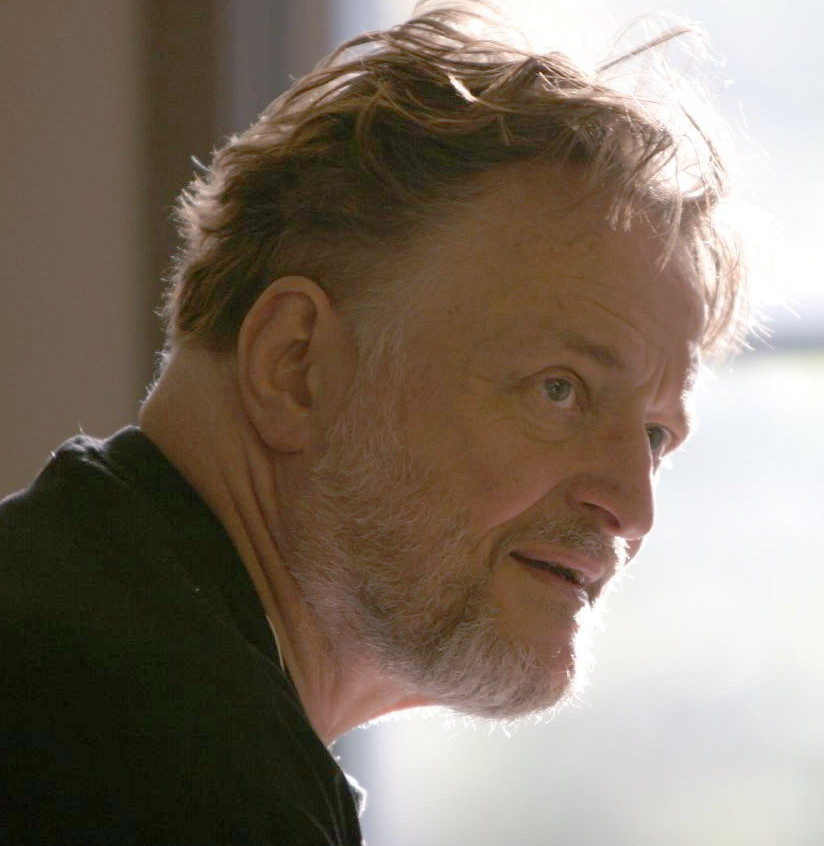
\includegraphics[width=0.9\textwidth]{conway} \\
		John H. Conway
% CC-BY: Thane Plambeck: http://www.flickr.com/photos/thane/20366806/
	\end{column}

	\begin{column}{0.5\textwidth}
		\centering
		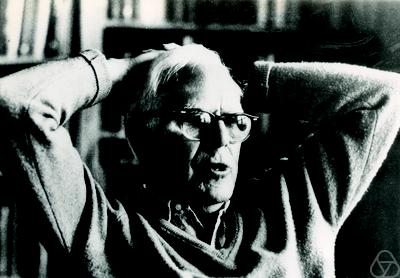
\includegraphics[width=0.9\textwidth]{gardner} \\
		Martin Gardner
% CC-BY-SA: http://owpdb.mfo.de/detail?photo_id=1292
	\end{column}
	\end{columns}
\end{frame}
\end{comment}

\begin{frame}{The game of Life}
	\begin{itemize}
		\item From these simple rules, complicated and unpredictable behaviour arises
		\item We can make sense of the behaviour by looking at individual stable patterns
		\item Our aim is to build up a pattern sufficiently complicated that it can do `useful' computation
	\end{itemize}
\end{frame}

\begin{frame}{Some stable patterns}{Still lifes}
	\game{still1}{2}
	Still lifes have period 1.
\end{frame}

\begin{frame}{Some stable patterns}{Blinkers}
	\game{blinker}{3}
	This blinker has period 2.
\end{frame}

\begin{frame}{More complex behaviour}{Gliders}
	\game{glider}{8}
	The glider shape has period 4, but moves from its original position.
\end{frame}

\begin{frame}{More complex behaviour}{Glider versus glider}
	\game{glidervs}{4}
	When two gliders collide, they annihilate each other.
\end{frame}

\begin{frame}{More complex behaviour}{Eaters}
	\game{eater}{6}
	The eater is a still life, and destroys an oncoming glider in 4 turns.
\end{frame}

\begin{comment}
\begin{frame}{How complex can we go?}
% http://ddi.cs.uni-potsdam.de/HyFISCH/Produzieren/lis_projekt/proj_gamelife/ConwayScientificAmerican.htm
	\begin{block}{Conjecture (Conway, 1970)}
		There does not exist a finite initial configuration such that the number of live cells after $n$ turns goes off to infinity.
	\end{block}
	\medskip

%	\pause
%	\begin{itemize}
%		\item Disproved shortly afterwards by Gosper (1970)
%		\item In fact, a much more interesting result was later shown by Conway himself (1982)
%	\end{itemize}
\end{frame}
\end{comment}

% best source I can find for date: http://gosper.org/bill.html
\begin{frame}{How complex can we go?}{Unbounded growth: Gosper's glider gun}
	\imseq{Turn \theturn\\\medskip}{gosper}{0,3,...,42,45}
	The Gosper glider gun has period 30, producing a glider on the 15th turn in each cycle.
\end{frame}

\begin{frame}{How complex can we go?}
	\pause
% see Rendell (2014)
	\begin{block}{Theorem}
		Life is Turing-complete.
	\end{block}

	\pause
	\begin{center}
		\rotatebox{90}{$\iff$}
	\end{center}

	\begin{block}{Theorem}
		If anything else can compute the result of a given function, so can Life.
	\end{block}
\end{frame}

%\begin{frame}{Logic gates}
%	\begin{itemize}
%		\item Many ways of modelling computation in Life have been discovered
%		\item Modern digital computer chips are built from billions of logic gates
%		\item Constructing logic gates in Life will give us a means to compute things
%	\end{itemize}
%\end{frame}

\begin{frame}{Logic gates}
	\pause
	\begin{itemize}
		\item Boolean functions operate on two values: \on and \off
		\item Can express all such functions as combinations of $\mathsf{NOT}$ and $\mathsf{AND}$ 
	\end{itemize}

	\bigskip
	\begin{columns}[onlytextwidth]
		\begin{column}{0.5\textwidth}
			\centering
			\begin{tabular}{c|c}
				$a$ & $\mathsf{NOT}~ a$ \\
				\hline
				\on & \off \\
				\off & \on
			\end{tabular}
		\end{column}

		\begin{column}{0.5\textwidth}
			\centering
			\begin{tabular}{c|c|c}
				$a$ & $b$ & $a ~\mathsf{AND}~ b$ \\
				\hline
				\on & \on & \on \\
				\on & \off & \off \\
				\off & \on & \off \\
				\off & \off & \off
			\end{tabular}
		\end{column}
	\end{columns}

%	\pause
%	\medskip
%	\begin{itemize}
%		\item Any Boolean function can be expressed as a combination of these gates
%		\item We can do binary arithmetic with Boolean functions
%	\end{itemize}
\end{frame}

\begin{comment}
\begin{frame}{Logic gates}{NAND}
	\begin{itemize}
		\item If we glue together an AND gate and then a NOT gate, we get a NAND gate
	\end{itemize}

	\begin{center}
		\begin{tabular}{c|c|c}
			$a$ & $b$ & $a ~\mathsf{NAND}~ b$ \\
			\hline
			\on & \on & \off \\
			\on & \off & \on \\
			\off & \on & \on \\
			\off & \off & \on
		\end{tabular}
	\end{center}

	\pause
	\begin{itemize}
		\item It turns out any Boolean function can also be expressed as a combination of NANDs
	\end{itemize}
\end{frame}

\begin{frame}{Bringing gates to Life}
	\begin{itemize}
		\item Build a `circuit' where gliders act like electrons carrying current
		\item Just like in a real circuit, gliders present represents \on; no glider means \off
		\item We use glider guns as current sources
		\item We can use interactions with other patterns (such as eaters) to selectively destroy gliders and produce \off{}s
	\end{itemize}
\end{frame}
\end{comment}

\begin{frame}{Bringing gates to Life}{Encoding input}
	\begin{columns}%[onlytextwidth]
	\begin{column}{0.7\textwidth}
		\begin{itemize}
			\item We encode a series of bits as a line of gliders
			\item A glider represents \on
			\item We leave a space to represent \off
			\item Timing must be perfect: a glider moves 1 cell every 4 turns
		\end{itemize}
	\end{column}

	\begin{column}{0.4\textwidth}
		\begin{center}
			\includegraphics[width=\textwidth,height=\textheight,keepaspectratio]{bitstream-0} \\
			The bit stream '\on~\on~\off~\on'
		\end{center}
	\end{column}
	\end{columns}
\end{frame}

\begin{frame}[t]{Bringing gates to Life}{The NOT gate}
	\begin{itemize}
		\item A glider gun continually makes gliders aimed so they collide with the input bitstream
		\item If the current bit is \on, the gliders annihilate each other, producing \off
		\item If it is \off, the glider from the gun can pass, giving \on
	\end{itemize}

	\begin{center}
		\begin{tikzpicture}
			\draw[->,thick] (-2,2) -- (-0.1,0.5) node[pos=-.2] {Glider gun};
			\draw[->,thick] (4,2) -- (2.1,0.5) node[pos=-.2] {Input bit $x$};
			\draw (0,0) rectangle (2, 1) node[pos=.5] {Collision};
			\draw[->,thick] (1,-0.1) -- (1,-0.75) node[pos=1.5] {NOT $x$};
		\end{tikzpicture}
	\end{center}
\end{frame}

\begin{frame}[t]{Bringing gates to Life}{The AND gate}
	\begin{columns}
	\begin{column}{0.5\paperwidth}
		\begin{itemize}
			\item Collide both bitstreams in sequence
			\item If both are \on, the \on from input $x$ consumes the gun glider leaving $y$ free to be output
			\item If only one is \on, it will consume the gun glider leaving no gliders left as output
			\item If both are \off, the gun glider keeps moving in the wrong direction, where it is tidied up by an eater
		\end{itemize}
	\end{column}

	\begin{column}{0.5\paperwidth}
		\begin{center}
			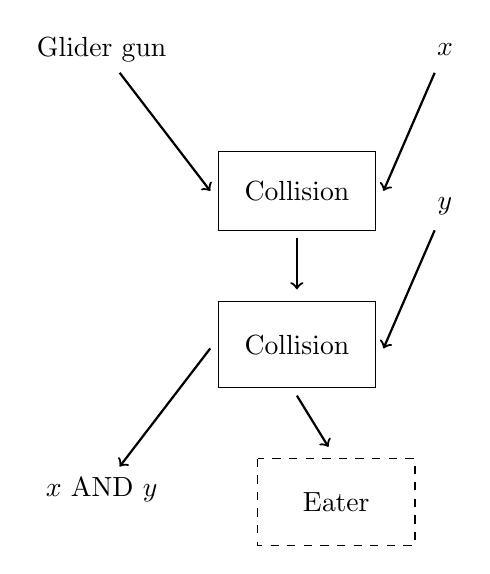
\begin{tikzpicture}
				\draw[->,thick] (-1.25,2) -- (-0.1,0.5) node[pos=-.2] {Glider gun};
				\draw[->,thick] (2.75,2) -- (2.1,0.5) node[pos=-.2] {$x$};
				\draw (0,0) rectangle (2, 1) node[pos=.5] {Collision};
				\draw[->,thick] (1,-0.1) -- (1,-0.75);
				\draw[->,thick] (2.75,0) -- (2.1,-1.5) node[pos=-.2] {$y$};
				\draw (0,-0.9) rectangle (2, -2) node[pos=.5] {Collision};
				\draw[->,thick] (1,-2.1) -- (1.4,-2.75);
				\draw[dashed] (0.5,-2.9) rectangle (2.5, -4) node[pos=.5] {Eater};
				\draw[<-,thick] (-1.25,-3) -- (-0.1,-1.5) node[pos=-.2] {$x$ AND $y$};
			\end{tikzpicture}
		\end{center}
	\end{column}
	\end{columns}
\end{frame}

\begin{frame}{Turing-completeness}
	\begin{itemize}
		\item We can embed any finite logic circuit in Life
			\begin{itemize}
				\item For example, a computer CPU
			\end{itemize}
		\item Can represent the transition function of a Turing machine in this way
		\item A combination of gliders and still lifes can act as memory
		\item With some machinery, we then have a full Turing machine
	\end{itemize}
\end{frame}

\begin{frame}{Turing-completeness}
	\begin{columns}
		\begin{column}{0.3\paperwidth}
		\begin{itemize}
% http://rendell-attic.org/gol/tm.htm
			\item Rendell (2000) built an `actual' Turing machine pattern in Life
			\item Grid dimensions are 1,714~$\times$~1,647
% http://rendell-attic.org/gol/utm/index.htm
			\item Rendell later (2010) built a Universal Turing Machine
		\end{itemize}
	\end{column}

	\begin{column}{0.7\paperwidth}
		\begin{center}
			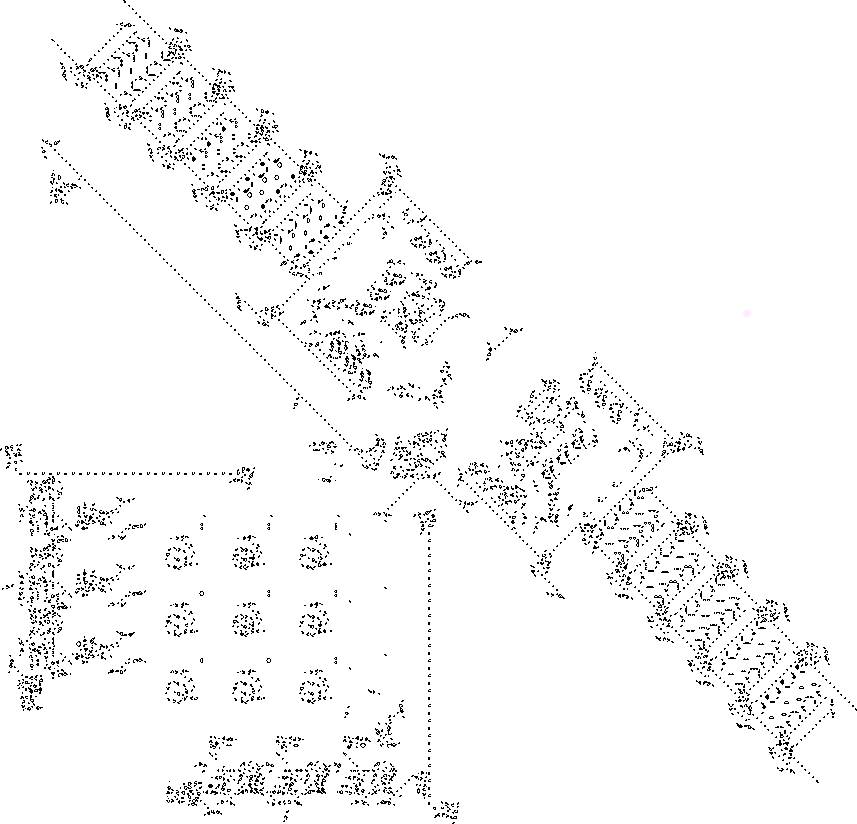
\includegraphics[width=\textwidth,height=0.65\textheight,keepaspectratio]{rendell-tm}
		\end{center}
	\end{column}
	\end{columns}
\end{frame}

\begin{comment}
\begin{frame}{Variations on a theme}
	\begin{itemize}
		\item Life is one of a family of games called `cellular automata'
		\item There are a number of Life-like automata which change the number of neighbours required for a cell to live or die
% http://www.complex-systems.com/pdf/15-1-1.pdf
		\item Cook (2004) showed that even the 1-dimensional Rule 110 automaton is Turing-complete
% http://arxiv.org/abs/1111.1567
		\item Rafler (2011) formulated SmoothLife, a continuous version of Life
	\end{itemize}
\end{frame}
\end{comment}

\end{document}
